\graphicspath{ {Context/Images/} }


\chapter{Context}
\label{cha:context}

\section{Introduction}
In this chapter 

Context: Depends on chosen problem (Extracting knowledge from EHR )

	Problem: info out of EHR
	State of the art:
	
		Explain Disease codes
		DiseaseProgression
		Explain Danish paper, Matrix group America (recommender), Querying


\section{Electronic Health Records}

An electronic health records (EHR) is a collection of data about a patient at a certain point in time. It is stored digitally and thus can be part of a large number of patients over a long time period.

\subsection{Disease Codes}

An important part of EHRs is applying methods which are uniform and well documented. This makes it easy to store and extract data from large-scale databases of EHRs. A part of an EHR consists of the diagnosis of the patient. It provides information about the disease trajectory of the patient and allows analysis on the health situation of a patient. With a uniform system for classifying diseases, it is possible to provide a general picture on health situations of populations.

\subsubsection{ICD-10}

The International Statistical Classification if Diseases and Related Health Problems (ICD) is a medical classification list made by the World Health Organization (WHO). The ICD contains more than $14,400$ codes about diseases, disorders, injuries, and other related health conditions. It also provides hierarchical categories for those codes to allow a more general overview of diseases.


\subsubsection{MedDRA}

The Medical Dictionary for Regulatory Activities (MedDRA) provides medical terminology in the form of disease codes. It doesn't provide hierarchical categories.

\section{EHR Analytics}

EHRs provide a massive amount of data which could be used to create useful insights. Those insights can be offered on an individual level, which means a right intervention to the right patient at the right time. EHR analytics can be used to have a personalized care for patients and benefits the healthcare system by cutting costs and improved outcomes. \\

In the following sections we talk about current EHR analytic methods.


\subsection{Querying}

Analytics on EHRs is still done through querying a database. A specialist can have a certain idea about correlations between conditions or patients. He can support this idea by finding cases in EHRs for example. \\
This method is based on the knowledge and experience of a specialist. The information has to be actively be sought after and thus a lot of other information is never found. Also complex relations aren't easily found and maybe too subtle to be found by a querying language.

\subsection{Recommender Systems}

An EHR of a patient can be transformed into a matrix structure, see figure \ref{fig:matrixPatient}. On these matrix structures, feature extraction methods can be applied similar to recommender systems. This can, for example, be done by defining patient similarities. So when a patient is similar to a previous patient, his treatment can be based on previous experiences.

\begin{figure}[H]
	\centering
	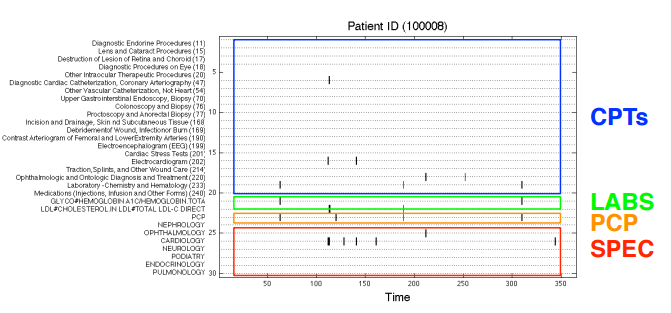
\includegraphics[width=8cm]{matrixPatient.png}
	\caption{An example of an EHR transformed into a matrix structure.}
	\label{fig:matrixPatient}
\end{figure}


\subsection{Statistical Analysis}

A combination of statistical methods and graph clustering are applied to obtain disease trajectories. To have any significance using those methods, a large set of EHRs need to be used. \\
These techniques have been applied to Danish EHRs. The study identifies temporal correlations between pairs of diagnoses. The pairs are further clustered into larger disease trajectories based on the diagnoses they shared. Based on the clusters, patients can be categorized into certain trajectories and retrieve a more personal care. An example of a cluster graph can be found in figure \ref{fig:clusterGraphDanish}.

\begin{figure}[H]
	\centering
	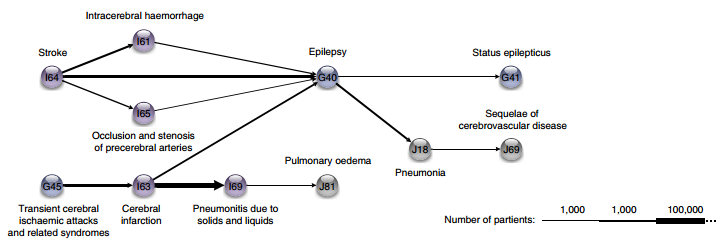
\includegraphics[width=8cm]{clusterGraphDanish.png}
	\caption{A cerebrovascular disease trajectory cluster for the Danish population.}
	\label{fig:clusterGraphDanish}
\end{figure}



http://www.who.int/classifications/icd/en/

http://arxiv.org/pdf/1112.1668v1.pdf

https://en.wikipedia.org/wiki/Electronic\_health\_record\#Technical\_features

file:///media/milan/Data/Chrome\%20Downloads/EHRAnalytics\_Stateoftheart\%20(1).pdf

http://www.meddra.org/

https://www.siam.org/meetings/sdm13/sun.pdf

Jimeng Sun, Fei Wang, Jianying Hu, Shahram Edabollahi: Supervised patient similarity measure of
heterogeneous patient records. SIGKDD Explorations 14(1): 16-24 (2012)

https://books.google.co.uk/books?id=eZmjIVtVtucC\&pg=
PA96\&lpg=PA96\&dq=querying+ehr\&source=bl\&ots=
AM3VVXy\_n-\&sig=epPrp87M\_ZixVmikVJKto8IvyIM\&
hl=nl\&sa=X\&ved=0ahUKEwjQ3MzouPrLAhXFhQ8KHaqs
D5I4ChDoAQgbMAA\#v=onepage\&q=querying
\%20ehr\&f=false

Towards Heterogeneous Temporal Clinical Event Pattern
Discovery:A Convolutional Approach


http://www.nature.com/ncomms/2014/140617/ncomms5022/pdf/ncomms5022.pdf


\section{Conclusion}
The final section of the chapter gives an overview of the important results
of this chapter. This implies that the introductory chapter and the
concluding chapter don't need a conclusion.



%%% Local Variables: 
%%% mode: latex
%%% TeX-master: "thesis"
%%% End: 
